% الجزء: sets-functions-relations
% الفصل: relations
% القسم: graphs

\documentclass[../../../include/open-logic-section]{subfiles}

\begin{document}

\olfileid[ar]{sfr}{rel}{grp}
\olsection{الرسوم البيانية}

\emph{الرسم البياني} مخطط من نقاط تصل بينها حواف؛ وتسمى النقاط
«عقدًا» أو «رؤوسًا»، واحدها «رأس». والرسوم كثيرة الاستعمال في
الرياضيات المتقطعة وعلوم الحاسوب، لما تعين عليه من تمثيل العلاقات
والبنى وتصويرها: من الشبكات العيانية على اختلافها إلى البنى المجردة
كالنتائج الممكنة للقرارات. ولها في المراجع أنواع شتى؛ فمن حوافها
الموجه وغير الموجه، والموسوم وغير الموسوم، ومنها ما يجيز حافة من
العقدة إلى نفسها أو حواف عدة بين العقدتين، وغير ذلك.
وللرسوم \emph{الموجهة} خاصة صلة بالعلاقات.

\begin{defn}[الرسم البياني الموجه]
\emph{الرسم البياني الموجه} هو ${\OLId{latin-looped}{G}} = \tuple{{\OLId{latin-looped}{V}}, {\OLId{latin-looped}{E}}}$، حيث~${\OLId{latin-looped}{V}}$ مجموعة
\emph{الرؤوس}، و~${\OLId{latin-looped}{E}} \subseteq {\OLId{latin-looped}{V}}^{\OLMathNumeral{2}}$ مجموعة \emph{الحواف}.
\end{defn}

\begin{explain}
فالرسم بهذا التعريف مجموعة ومعها علاقة عليها. وتمثيله للعين أن
نصل الرأس~${\OLId{latin-ordinary}{v}}_{\OLMathNumeral{1}}$ بالرأس~${\OLId{latin-ordinary}{v}}_{\OLMathNumeral{2}}$ بسهم إذا وفقط إذا كان
$\tuple{{\OLId{latin-ordinary}{v}}_{\OLMathNumeral{1}}, {\OLId{latin-ordinary}{v}}_{\OLMathNumeral{2}}} \in {\OLId{latin-looped}{E}}$. وإنما يفارق الرسم العلاقة وحدها بأنه
يصرح بمجموعة الرؤوس، فيجوز أن يحتوي رؤوسًا معزولة. والحاصل أن كل
علاقة~${\OLId{latin-looped}{R}}$ على مجموعة~${\OLId{latin-looped}{X}}$ تؤخذ رسمًا موجهًا $\tuple{{\OLId{latin-looped}{X}}, {\OLId{latin-looped}{R}}}$؛ وبالعكس
يؤخذ الرسم الموجه~$\tuple{{\OLId{latin-looped}{V}}, {\OLId{latin-looped}{E}}}$ علاقة ${\OLId{latin-looped}{E}} \subseteq {\OLId{latin-looped}{V}}^{\OLMathNumeral{2}}$ صرح
بمجموعة ${\OLId{latin-looped}{V}}$ التي تقع عليها.
\end{explain}

\begin{ex}
لتكن صورة الرسم البياني $\tuple{{\OLId{latin-looped}{V}}, {\OLId{latin-looped}{E}}}$ الذي فيه ${\OLId{latin-looped}{V}} = \{{\OLMathNumeral{1}}, {\OLMathNumeral{2}}, {\OLMathNumeral{3}}, {\OLMathNumeral{4}}\}$ و${\OLId{latin-looped}{E}} =
\{\tuple{{\OLMathNumeral{1}},{\OLMathNumeral{1}}}, \allowbreak \tuple{{\OLMathNumeral{1}}, {\OLMathNumeral{2}}}, \allowbreak \tuple{{\OLMathNumeral{1}}, {\OLMathNumeral{3}}},
\allowbreak \tuple{{\OLMathNumeral{2}}, {\OLMathNumeral{3}}}\}$ على هذا الوجه:
\begin{align*}
& 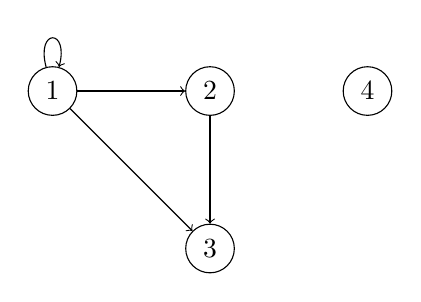
\begin{tikzpicture}[->,node distance=2cm]
  \node[draw,circle] (A) {${\OLMathNumeral{1}}$};
  \node[draw,circle] (B) [right of=A] {${\OLMathNumeral{2}}$};
  \node[draw,circle] (C) [below of=B] {${\OLMathNumeral{3}}$};
  \node[draw,circle] (D) [right of=B] {${\OLMathNumeral{4}}$};
  \draw (A) to [loop above]  (A);
  \draw (A) to  (B);
  \draw (A) to  (C);
  \draw (B) to  (C);
  \end{tikzpicture}
\intertext{وهذا رسم بياني مختلف عن $\tuple{{\OLId{latin-looped}{V}}', {\OLId{latin-looped}{E}}}$ الذي فيه ${\OLId{latin-looped}{V}}' =
  \{{\OLMathNumeral{1}}, {\OLMathNumeral{2}}, {\OLMathNumeral{3}}\}$، والذي يبدو كما يأتي:}
& 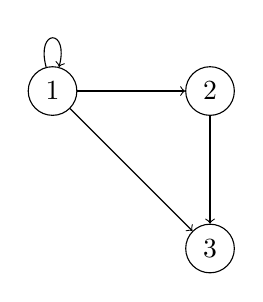
\begin{tikzpicture}[->,node distance=2cm]
  \node[draw,circle] (A) {${\OLMathNumeral{1}}$};
  \node[draw,circle] (B) [right of=A] {${\OLMathNumeral{2}}$};
  \node[draw,circle] (C) [below of=B] {${\OLMathNumeral{3}}$};
  \draw (A) to [loop above]  (A);
  \draw (A) to  (B);
  \draw (A) to  (C);
  \draw (B) to  (C);
  \end{tikzpicture}
\end{align*}
\end{ex}

\begin{prob}
خذ علاقة أصغر من أو يساوي~$\le$ على $\{{\OLMathNumeral{1}},
  {\OLMathNumeral{2}}, {\OLMathNumeral{3}}, {\OLMathNumeral{4}}\}$ رسمًا بيانيًا، ثم صوّرها بالمخطط الموافق.
\end{prob}

\end{document}
